% !TeX encoding = UTF-8
% !TeX spellcheck = en_US
% !TeX root = ledgersmb-book.tex

\part{Configuration}
\label{part-configuration}


\chapter{Overview}
\label{cha-configuration-overview}

\section{Introduction}
\label{sec-config-overview-introduction}
This section of the book describes how to set up LedgerSMB and its components.
Configuration is assumed to be mostly one-off and rather technical in nature.  To find
out which tasks might need to be performed in order to keep the application in good
health the reader is referred to the section ``Administration''. 

\chapter{Global configuration}
\label{cha-global-configuration}

\section{Apache}
\label{sec-global-config-apache}

Section about installing on Apache 2+

items to be discussed:

Forwarding of authentication \\
PSGI configuration \\
performance: cgiD configuration: don't (yet) [but will be supported once all legacy code is gone] \\
security: suEXEC environment \\

\subsection{Differences between Apache 1.3 and 2+}
\label{subsec-global-config-apache-13-vs-2}

Explain how to use lsmb with 1.3 instead of 2+.

\section{PostgreSQL}
\label{sec-global-config-postgresql}

pg\_hba.conf: authentication \\
security: local vs IP connections \\




\section{LedgerSMB}
\label{sec-global-config-ledgersmb}

LedgerSMB configuration using 'ledgersmb.conf' is deprecated as of 1 Jan 2023. New functionality may only available when using `ledgersmb.yaml` configuration file.

For the time being there is a conversion step that converts the old 'ledgersmb.conf' to `ledgersmb.yaml`, but the old conf file does not support new functionality.

\subsection{ledgersmb.yaml}
\label{subsec-global-config-ledgersmb-yaml}



\chapter{Per company configuration}
\label{cha-company-config}

\section{Matching your business processes}
\label{sec-company-config-matching-your-business}

By default, LedgerSMB operates such that all optional functionality is available and the user decides to use it or not based on which menu items they select, what fields they enter data into, and what buttons they click.

Removing application roles \index{application roles} (see \appref{app-role-listing}) can limit the visibility of  menu items, data fields, and buttons. This will simplify the users view of the system, reduce training, and better configure LedgerSMB to your business requirements.

Outside of application roles, the only other enforced business process configuration is whether the same person can both create and post transactions. It is called 'separation of duties' \index{separation of duties} and is defined in \secref{subsubsec-company-config-defaults-separation-of-duties}.

LedgerSMB is configured to adjust inventory \index{inventory} when a Sales or Purchase Invoice is posted. This closely matches retail business processes where the customer walks out of the establishment with the product and an invoice \index{invoice} (or receipt).  This functionality can also be used for wholesale shipping applications because LedgerSMB can also produce picking \index{picking} and \index{shipping} shipping documents, just remember that the inventory transaction happens when an invoice is posted.

LedgerSMB uses \gls{FIFO} \index{FIFO} for \gls{COGS} \index{COGS} and inventory calculations.  There are provisions for alternatives, but the code is not yet complete. See \secref{sec-accounting-valuation-inventory} for a detailed explanation of  \gls{FIFO} calculations.

In addition to the above, LedgerSMB has configurable Workflows \index{workflows}. These are not user configurable but your technical support staff should be able to create and edit them. See \charef{part-workflows}.

Contact the \href{https://ledgersmb.org}{development team} for other business process customizations.  In most cases the need for more flexible matching of LedgerSMB to your business processes is understood, but the project has not not yet had any customer requests or development volunteers.

\section{Administrative user}
\label{sec-company-config-admin-user}

\section{Chart of accounts}
\label{sec-company-config-coa}

@@@ Should refer to the 'administration' section???

\subsection{Special accounts}
\label{subsec-company-config-coa-special-accounts}

\begin{itemize}
\item AR/AP summary accounts
\item 5 other special purpose accounts, see ``Defaults'' screen discussion
\item sales tax accounts
\end{itemize}


\section{System menu settings}
\label{sec-company-config-system-menu}

This section enumerates the ``System'' menu's immediate children. In some cases the
functionality is too complex and is referred to a chapter of its own.

\subsection{Audit control}
\label{subsec-company-config-audit-control}

\subsubsection{Enforce transaction reversal for all dates}
\label{subsubsec-company-config-audit-control-reversals}


This is a Yes/No value which affects the actions which can be performed on posted financial transactions.
\begin{itemize}
\item No means transactions can be altered or deleted, even after posting them. Note that
if a transaction has been posted before the latest closing date, it can never be altered,
not even when this value is in effect.
\item Yes means transactions can't be altered after posting. This setting is highly preferred and considered the only correct approach to accounting as it assures visible
audit trails and thereby supports fraud detection.
\end{itemize}

\subsubsection{Close books up to}
\label{subsubsec-company-config-audit-control-close-books}


@@@ This item isn't a system setting; shouldn't it move to ``Transaction approval''?? That way system settings (config) and processes are separated.

@@@ My preference is to remove the setting entirely and rely on year-end 
workflow.  We might add an account checkpoint interface as well at some point
--Chris T

It's advisable to regularly close the books after review. This prevents user error changing
reviewed numbers: after closing the books, it's no longer possible to post in the closed
period.

There are also performance benefits to closing the books, because LedgerSMB uses the
fact that the figures are known-stable as a performance optimization when calculating
account balances.

\subsubsection{Activate audit trail}
\label{subsubsec-company-config-audit-control-audit-trail}

This is a Yes/No value which - when Yes - causes the system to install triggers to register
user actions (creation/adjustments/reversals/etc...) executed on financial transactions.


@@@ Once activated, where can we see it the audit trail??

@@@ This setting should go.  In 1.3 the audit trails are always enforced via
triggers so this setting does nothing.  --CT

\subsection{Taxes}
\label{subsec-company-config-taxes}


This page lists all accounts which have the ``Tax'' account option enabled as discussed in \secref{sec-coa-account-options}.

Each account is listed at least once, but can be listed many times, if it has had different
settings applied over different time periods. E.g. if one of the current VAT rates is 19\%,
today but it used to be 17.5\% until last month, there will be 2 rows for the applicable
VAT account. See \charef{cha-taxes} for further discussion of how taxes work in
LedgerSMB and the choices involved when being required to handle changes in tax rates.

Each row lists the following fields:

\begin{description}[style=nextline]
\item [Rate (\%)] The tax rate to be applied when calculating VAT to be posted on this account.
\item [Number] Account number
\item [Valid To] The ending date of the settings in this row. This can apply to the rate as well as the ordering or the tax rules (but usually applies to the rate).
\item [Ordering] This has to do with cumulative taxes.  For example if two taxes
exist and one has an ordering of 0 and one of 1, then the second tax will be
calculated on a basis that includes the first.  One place where this used to be
used was in Quebec, where GST was taxable under PST.
\item [Tax rules] LedgerSMB features a flexible structure to facilitate complex tax
calculations (see \secref{sec-tax-rule-plugins}). By default the ``Simple'' module
is the only one installed.
\end{description}

\subsection{Defaults}
\label{subsec-company-config-defaults}

\subsubsection{Business number}
\label{subsubsec-company-config-defaults-business-number}
   This is used to store an arbitrary identification number for the business.  It
could be used to store a business license number or anything similar.
   
\subsubsection{Weight unit}
\label{subsubsec-company-config-defaults-weight-unit}
   The unit of measurement for weights. @@@ why don't we have a unit of measurement for distance as well??? And maybe a unit of measurement for content?
   
\subsubsection{Separation of duties}
\label{subsubsec-company-config-defaults-separation-of-duties}

% For better or worse this is the spot for the canonical definition of separation of duties.

Separation of duties \index{separation of duties} is a method to help reduce fraud where one employee can't modify the
accounting ledger without another employee's approval.

Select "Yes" if you want to activate separation of duties or "No" if you don't
want to activate it.

In order for separation of duties to be enforced, user roles have to be set differently for each user. This is done by removing the \texttt{draft\_post} role from the users that cannot post and making sure that the users that can post have the role enabled.  See \secref{sec-user-management-authorization} for more details about changing and setting User Roles.

\subsubsection{Default accounts}
\label{subsubsec-company-config-defaults-accounts}

This setting will be used to preselect an account in
the listings of the three categories listed below:
\begin{itemize}
\item Inventory
\item Income
\item Expense
\end{itemize}


\subsubsection{Foreign exchange gain and loss accounts}
\label{subsubsec-company-config-defaults-fx-accounts}

When working with foreign currencies,
the system needs two special purpose accounts. One to post the gains onto which are
caused by foreign currencies increasing in value; the other to post the losses onto
which are caused by foreign currencies decreasing in value.


\subsubsection{Default country}
\label{subsubsec-company-config-defaults-country}

This setting indicates which country needs to be pre-selected
   in country selection lists.


\subsubsection{Default language}
\label{subsubsec-company-config-defaults-language}

The language to be used when no other language has been selected. Several parts of the
application require language selection, such as customer, vendor and employee entry screens.

\subsubsection{Templates directory}
\label{subsubsec-company-config-defaults-templates}

This setting indicates which set of templates - stored in the
   \texttt{templates/} directory - should be used. In a standard installation, the drop down
   lists two items:
\begin{description}[style=nextline]
   \item [demo] which contains templates based on \LaTeX, which is more commonly installed but has issues dealing with accented characters
   \end{description}


\subsubsection{List of currencies \& default currency}
\label{subsubsec-company-config-defaults-currencies}

Enter a list of all currencies you want
to use in your company, identified by their 3-letter codes separated by a colon; i.e.
``USD:EUR:CHF''. To ensure correct operation of the application, at least one currency
(the company default currency) must be listed. In case of multiple currencies the first
is used as the company default currency.

\subsubsection{Company data (name /address)}
\label{subsubsec-company-config-defaults-name-address}

The fields ``Company Name'', ``Company Address'',
``Company Phone'' and ``Company Fax'' will be used on printed/e-mailed invoices.

\subsubsection{Password duration}
\label{subsubsec-company-config-defaults-password-duration}

This is an integer value field measuring the validity period in days for passwords set through
the user's \texttt{Preferences} screen. If this field is empty, passwords set through that method
won't expire.

A user will receive password expiration reminders upon logging starting a week before password
expiry. When not acted upon, starting two days before expiry an hourly popup will appear
requesting the user to change the password.

The application behaves this way because users with expired passwords won't be able to log in:
their password will need to be reset by a user admin.

\begin{quotation}
Note that passwords set by admins for other users expire within 24 hours after setting them.
This value is hard coded and can't be overruled. This is a security measure taken to make
sure as few unused accounts as possible exist: Existence of such accounts could open up security
holes.
\end{quotation}


\subsubsection{Default E-mail addresses}
\label{subsubsec-company-config-defaults-email}

These addresses will be used to send e-mails from the system.
Note that the ``Default Email From'' address should be configured in order to make sure
e-mail doesn't look like it's coming from your webserver. The format to be used is \texttt{``Name'' <e-mail address>} where the e-mail address should be inserted between the
``$\langle$'' and ``$\rangle$''.

\subsubsection{Max per dropdown}
\label{subsubsec-company-config-defaults-max-dropdown}

Some elements in the screens may present a drop down. However, drop downs are
relatively unwieldy to work with when used to present a large number of values
to choose from.

This configuration option sets an upper limit on the number of records to be
presented as drop down.  When the number is exceeded, no drop down is used.  Instead,
a multi-step selection procedure will be used.

\subsubsection{Item numbering}
\label{subsubsec-company-config-defaults-item-numbers}

Many items in the system have sequence numbers: invoices, parts, etc.
These \index{sequence numbers} can be just a number (i.e. 1 or 37) or
they can also be both prefixed and suffixed. For example, INV0001 for invoices and EMP001 for employees or YOU-0001TOO, in which case the next item will be YOU-0002TOO. 

You can only issue every number in the sequence once, but you can issue Y21-001 and Y22-001 by changing the sequence number format at the beginning of the year.

The numbers shown in the input boxes will be used to generate the next number in the
numbering sequence.

\begin{description}[style=nextline]
\item [GL Reference number] The default reference number for the next GL transaction.
\item [Sales invoice/ AR Transaction number] This number is used to generate an invoice
number when none is being filled out by the user.
\item [Sales order number ] Same as Sales invoice number, except that it's used for sales orders @@@ layout issue: the label is too big to fit on the page
\item [Vendor invoice/ AP Transaction number] Same as Sales invoice, except that the number
is used for accounts payable transactions. @@@ layout issue: the label is too big to fit on the page 
\item [Sales quotation number] Same as sales order number, except that it's used for quotations.
\item [RFQ number] Request for quotation number is like the sales quotation number, except
that it is used to track which vendors have been asked for quotes.
\item [Part number] All parts, services and assemblies are identified by a unique number.
When an item is created and no number is entered by the user, a number is generated
from this sequence.
\item [Job/project number] Used when creating new projects.
\item [Employee number ] Same as the sales invoice number, used by new employee entry.
\item [Customer number] @@@ is this the control code number? or is this
meta\_number?? -- Meta-number (CT) 
\item [Vendor number] @@@ same question as customer number
\end{description}

\subsubsection{Check prefix}
\label{subsubsec-company-config-defaults-check-prefix}

 The prefix to use when printing checks. There's no check sequence number. That sequence number is requested from the check printing interface, because
checks can be created outside the application as well, meaning the numbers can
get out of sync.

\subsection{Year end}
\label{subsec-company-config-year-end}

@@@ Rename ``Yearend'' in menu interface to ``Year end''.


@@@ IMO this section doesn't belong here, because it's a process, not config, but does it belong in this menu then? IMO it doesn't...


\subsection{Admin users}
\label{subsec-company-config-admin-users}

@@@ Same as Year end; doesn't belong here...

\subsection{Chart of accounts}
\label{subsec-company-config-coa}

@@@ Chart of accounts isn't exactly a ``process'', but it doesn't feel like being pure
config either. At any rate it's a fact that the CoA discussion is a full chapter in and
of itself - so discussion here isn't necessary anymore.

\subsection{Warehouses}
\label{subsec-company-config-warehouses}

Warehouses are stocking locations. They don't have any properties (in the system)
other than that they have a name. Warehouses can be added, modified and deleted from
the \menupath{System \ma Warehouses} menu item.

\subsection{Departments}
\label{subsec-company-config-departments}

Departments can be used to divide a company in smaller pieces. LedgerSMB distinguishes two
types of departments:

\begin{description}[style=nextline]
\item [Profit centers] which can be associated with any type of transaction, including AR transactions.
\item [Cost centers] which can be associated with all types of transactions, except AR transactions.
\end{description}

Departments can be created (added), modified or deleted through the \menupath{System \ma Departments} menu item.

\subsection{Type of business}
\label{subsec-company-config-business-types}

Types of business are used in sales operations where customers can be assigned a type
of business. Based on the type of business assignment, quotations, sales orders and
invoices will automatically apply discount rates. For each type of business you enter a description and a discount rate to be applied.

\subsection{Languages}
\label{subsec-company-config-languages}

The language table is the table users can select languages from, both to present
the UI of the application as well as the setting for customers to be used to generate
documents.

This listing should correspond to the actual translations of the application being
available in the program installation directory.

Languages can be added, modified or deleted through the \menupath{System \ma Language} menu item.

\subsection{Standard Industry Code (SIC)}
\label{subsec-company-config-sic}

SI codes feature these three fields:

\begin{description}
\item [Code]
\item [Heading]
\item [Description]
\end{description}

When creating a company you can assign that it an SIC code, irrespective of its role (i.e. customer,
vendor, lead or anything else). An example of an SI code system is the
US's NAICS\footnote{\url{https://www.census.gov/naics/}} code.
Other countries have their own coding systems such
as ANZSIC\footnote{\url{https://www.abs.gov.au/statistics/classifications/australian-and-new-zealand-standard-industrial-classification-anzsic/latest-release}} for Australia and New Zealand
and NACE\footnote{\url{https://ec.europa.eu/competition/mergers/cases/index/nace\_all.html}} for Europe

The SIC field currently doesn't support a specific function in the application and is there
merely for informational purposes. However in the future its role could be extended to include
impact on reports, taxes or other functionalities where type of industry could matter.

\subsection {Templates}
\label{subsec-company-config-templates}

Templates are available to control the output format of many LedgerSMB outputs including Balance Sheet, Sales Orders, etc.

There are 3 types of templates: \LaTeX, HTML, and CSV.
Templates are accessed by navigating to \menupath{System \ma Templates}.
You should see the view shown in \figref{fig:system-templates}.

The template you want to change is selected in the "Template" drop-down. The template format you want to change is selected in the "Format" drop-down.

\begin{figure}[h]
        \centering
        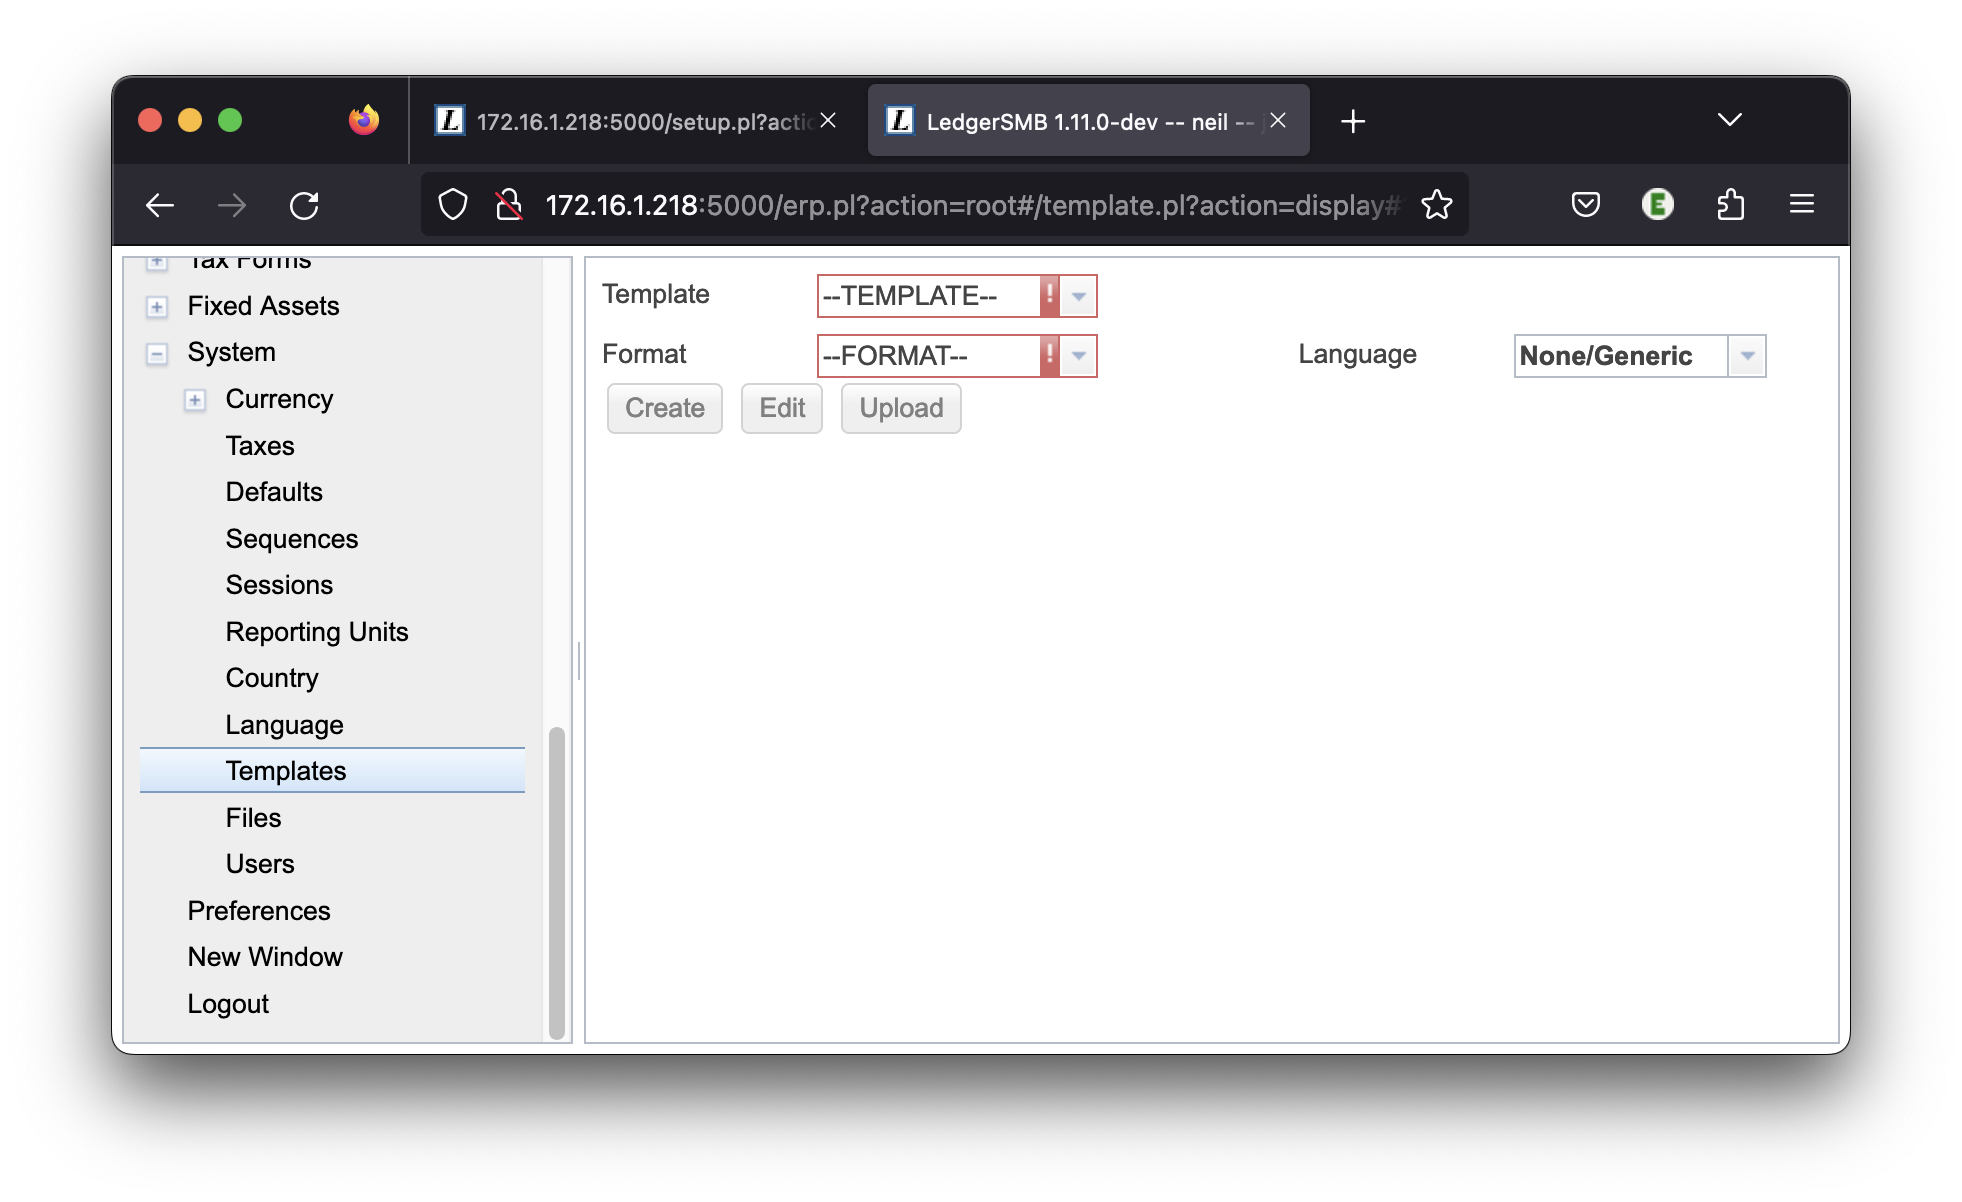
\includegraphics[width=13cm]{system-templates.png}
        \caption{System templates screen}
        \label{fig:system-templates}
\end{figure}

\subsubsection{\LaTeX{} templates}
\label{subsec-company-config-latex-templates}

To change a \LaTeX{} template navigate to \menupath{System \ma Templates}.
Select, for example, Template "Invoice" and Format "tex", you should see the view shown in \figref{fig:system-templates-edit-invoice}

\begin{figure}[h]
        \centering
        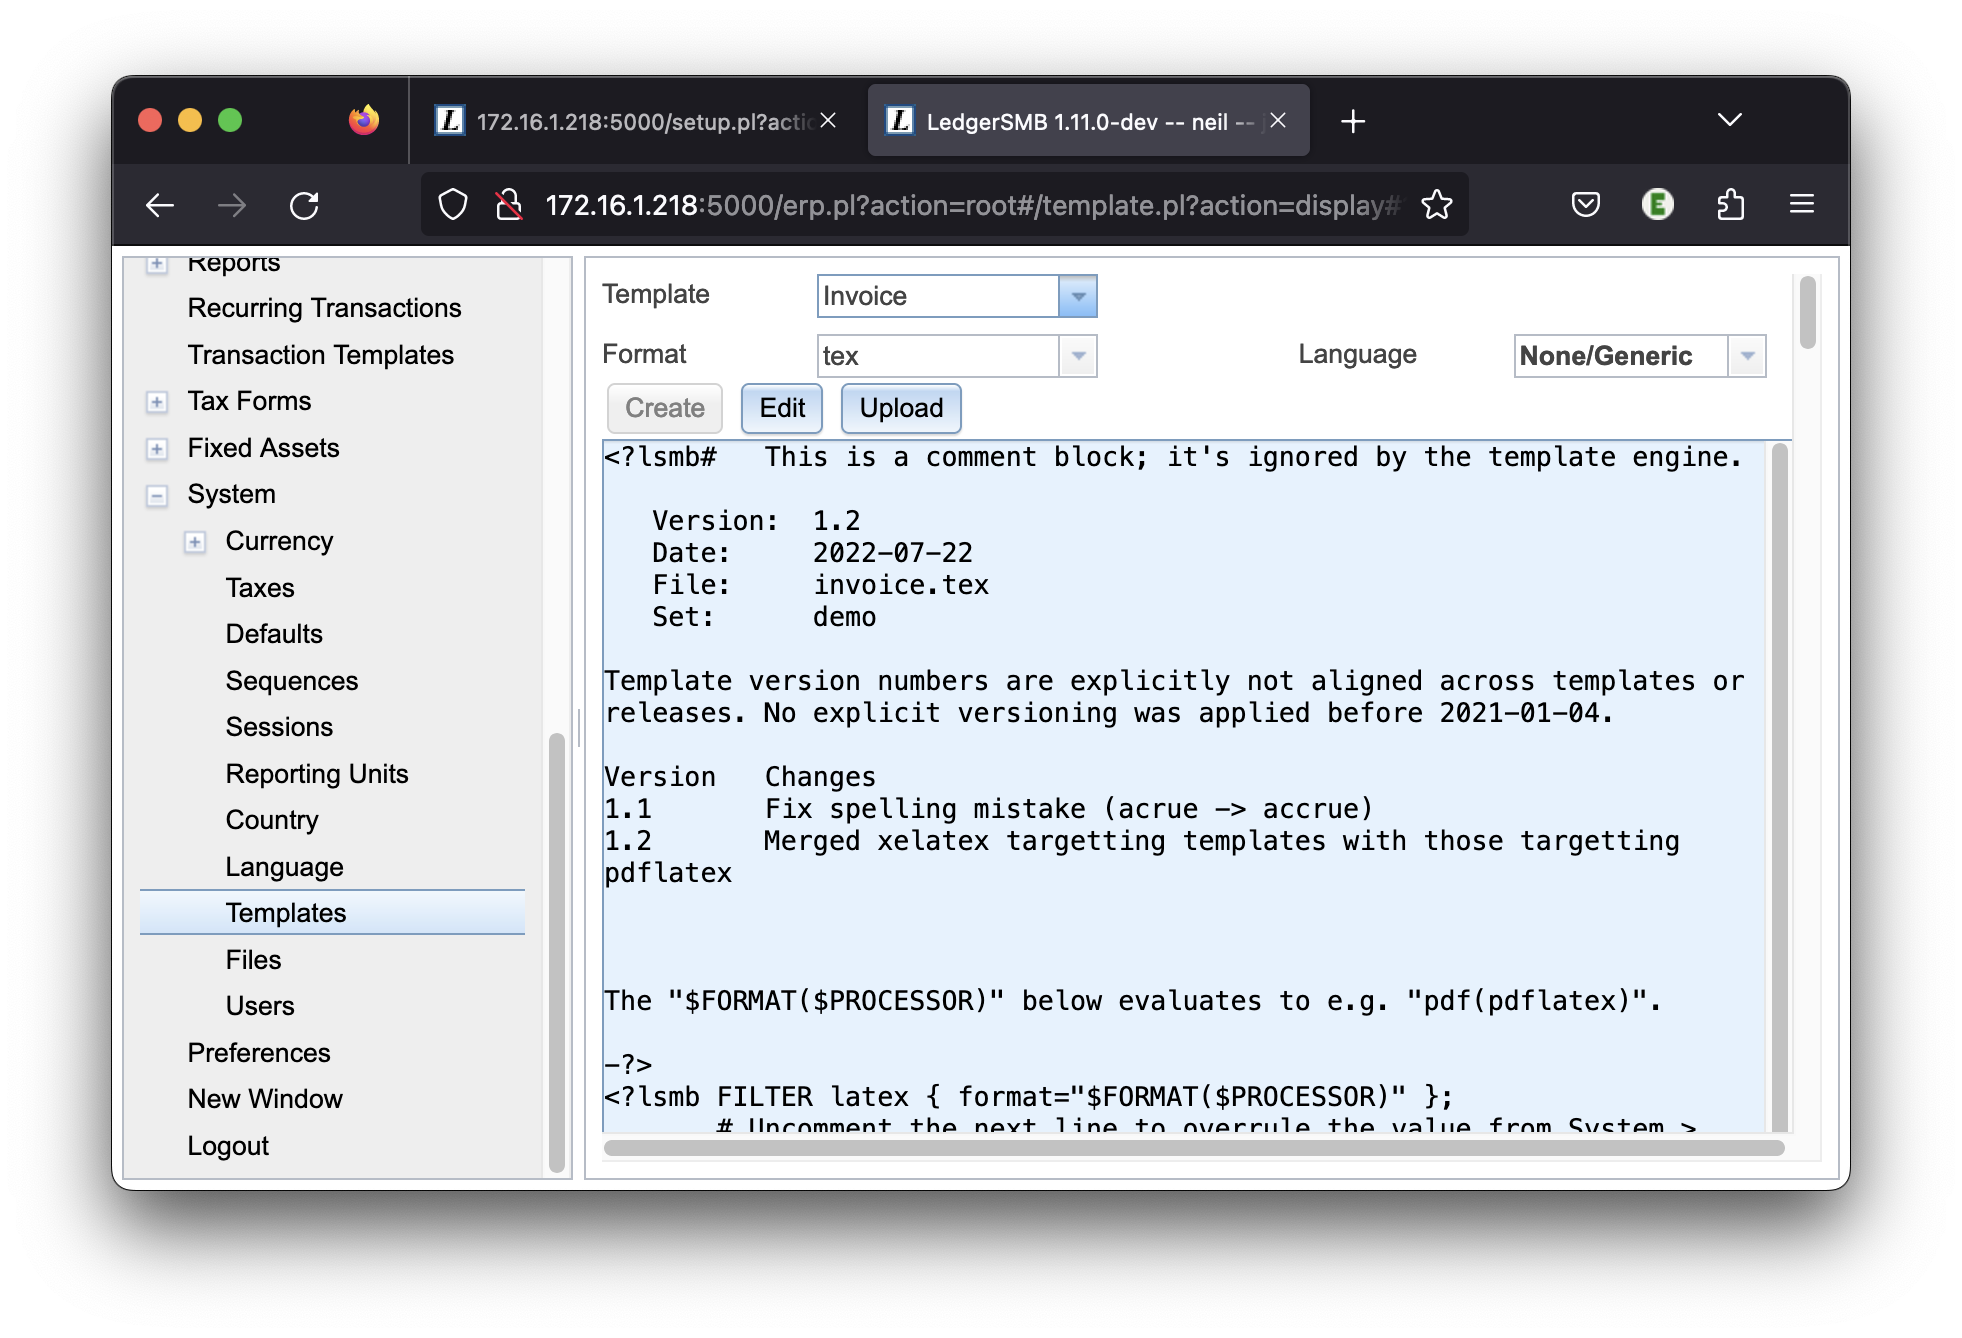
\includegraphics[width=13cm]{system-templates-edit-invoice.png}
        \caption{Templates edit invoice screen}
        \label{fig:system-templates-edit-invoice}
\end{figure}

To add a file to the latex template, first upload the image file to the database.  
This can be accomplished by navigating to \menupath{System \ma Files}.

To include this graphic file in your \LaTeX{} document, it needs to be retrieved from
the database and temporarily stored in a location accessible to the PDF
generator. Once the file is in the database, then the function \texttt{dbfile\_path} handles that.

For example, If the graphic file is named "FL\_Logo\_icon\_250x250.png", then add something like the following to the \LaTeX{} template using the \texttt{Edit} button.

\begin{verbatim}
\parbox[b]{.1\textwidth}{%
    \includegraphics[scale=0.7]{%
        <?lsmb dbfile_path("FL_Logo_icon_250x250.png")?>}
}
\end{verbatim}

After editing the template must be uploaded to the database using the \texttt{Upload} button.

\subsubsection{HTML templates}
\label{subsec-company-config-html-templates}

@@@TODO Add HTML specific template info.

\subsubsection{CSV templates}
\label{subsec-company-config-csv-templates}

@@@TODO Add CSV specific template information here.

